\begin{figure}
	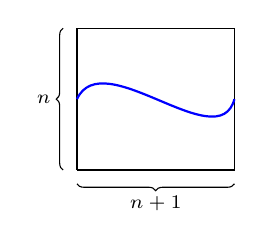
\begin{tikzpicture}[scale = 0.20]
		\draw (0, 0) -- (10, 0) -- (10, 9) -- (0, 9) -- (0, 0);
		\draw[decoration = {brace, mirror, raise = 5pt}, decorate] (0, 0) -- node[below = 6pt] {{\scriptsize $n + 1$ }} (10, 0);
		\draw[decoration = {brace, raise = 5pt}, decorate] (0, 0) -- node[left = 6pt] {{\scriptsize $n$ }} (0, 9);
		\draw[blue, thick] (0, 4.5) to[out = 65, in = -105] (10, 4.5);
	\end{tikzpicture}
	\vspace{-12pt}
	\caption{Evento $\HC(n+1, n)$.} 
	\label{fig-cruzamento-caixa}
\end{figure}